\documentclass[runningheads]{llncs}
\def\shownotes{1}
\def\notesinmargins{0}

%\usepackage{fullpage}
\usepackage{fancyvrb}
\usepackage{mathtools,color,xcolor,hyperref,graphicx,wrapfig,listings,array,xspace}
\usepackage{caption}
\usepackage{subcaption}
\usepackage{tikz}
\usetikzlibrary{arrows}

\usepackage{amsfonts}
% https://tex.stackexchange.com/questions/11719/how-do-i-backcolor-in-verbatim
\usepackage{xcolor}
\usepackage{alltt}
% Compensate for fbox sep:
\newcommand\Hi[2][lightgray]{%
	\hspace*{-\fboxsep}%
	\colorbox{#1}{#2}%
	\hspace*{-\fboxsep}%
}

\ifnum\shownotes=1
\ifnum\notesinmargins=1
\newcommand{\authnote}[2]{\marginpar{\parbox{\marginparwidth}{\small %
  \textsf{#1 {\textcolor{blue}{notes: #2}}}}}%
  \textcolor{blue}{\textbf{\dag}}}
\else
\newcommand{\authnote}[2]{
  \textsf{#1 \textcolor{blue}{: #2}}}
\fi
\else
\newcommand{\authnote}[2]{}
\fi

\newcommand{\snote}[1]{{\authnote{\textcolor{yellow}{Scalahub notes}}{#1}}}
\newcommand{\knote}[1]{{\authnote{\textcolor{green}{kushti notes}}{#1}}}


\newcommand{\ret}{\mathsf{ret}}
\newcommand{\new}{\mathsf{new}}
\newcommand{\hnew}{h_\mathsf{new}}
\newcommand{\old}{\mathsf{old}}
\newcommand{\op}{\mathsf{op}}
\newcommand{\verifier}{\mathcal{V}}
\newcommand{\prover}{\mathcal{P}}
\newcommand{\key}{\mathsf{key}}
\newcommand{\nextkey}{\mathsf{nextKey}}
\newcommand{\node}{\mathsf{t}}
\newcommand{\parent}{\mathsf{p}}
\newcommand{\leaf}{\mathsf{f}}
\newcommand{\vl}{\mathsf{value}}
\newcommand{\balance}{\mathsf{balance}}
\newcommand{\lft}{\mathsf{left}}
\newcommand{\rgt}{\mathsf{right}}
\newcommand{\lbl}{\mathsf{label}}
\newcommand{\direction}{\mathsf{d}}
\newcommand{\oppositedirection}{\bar{\mathsf{d}}}
\newcommand{\found}{\mathsf{found}}
\newcommand{\mypar}[1]{\smallskip\noindent\textbf{#1.}\ \ \ }
\newcommand{\ignore}[1]{}

\newcommand{\langname}{ErgoScript\xspace}
\newcommand{\powname}{Autolykos\xspace}
\newcommand{\poolname}{ErgoPool\xspace}
\newcommand{\mixname}{ErgoMix\xspace}
\newcommand{\zerocoin}{Zerocoin\xspace}


\newcommand{\lst}[1]{\text{\lstinline[basicstyle={\ttfamily}]$#1$}}

\newcommand{\andnode}{\ensuremath{\mathsf{AND}}}
\newcommand{\ornode}{\ensuremath{\mathsf{OR}}}
\newcommand{\tnode}{\ensuremath{\mathsf{THRESHOLD}}}

\newcommand{\GF}{\ensuremath{\mathrm{GF}}}


\begin{document}

\newcommand{\algname}{ZeroJoin\xspace}
\title{\algname: Combining \zerocoin and CoinJoin}

\author{Alexander Chepurnoy\inst{1,2}, Amitabh Saxena\inst{1}}

\institute{Ergo Platform \\\email{\{kushti\}@protonmail.ch, \{amitabh123\}@gmail.com} \and
IOHK Research \\\email{\{alex.chepurnoy\}@iohk.io}}

\maketitle

\begin{abstract}

We present \algname, a practical privacy-enhancing protocol for blockchain transactions. \algname can be considered a combination of \zerocoin and CoinJoin. 
Like \zerocoin, our protocol uses zero-knowledge proofs and a pool of
participants. However, unlike \zerocoin, our proofs are very efficient, and our pool size is not monotonically increasing.
Thus, our protocol overcomes the two major drawbacks of \zerocoin. Our approach can also be considered a non-interactive variant of CoinJoin, where the interaction is replaced by a public transaction on the blockchain. We also present \mixname, a practical implementation of \algname on top of Ergo, a smart contract platform based on Sigma protocols. While \algname contains the key ideas, it leaves open the practical issue of handling fees. The key contribution of \mixname is a novel approach to handle fee in \algname. 

\end{abstract}

\section{Introduction}
\label{intro}

Privacy enhancing techniques in blockchains generally fall into two categories. The first is hiding the amounts being transferred, such as in Confidential Transactions~\cite{ct}. The second is obscuring the input-output relationships such as in \zerocoin~\cite{zerocoin}, Monero~\cite{monero}, CoinJoin~\cite{coinjoin}, QuisQuis~\cite{quisquis} and Composite Signatures~\cite{composite}. Some solutions such as MimbleWimble~\cite{mw} and Zcash~\cite{zcash,zcash1} combine both.
%In fact, MW can be thought of as a combination of CT and OWAS.

In this work, we describe \algname, yet another privacy enhancing protocol based on the latter approach of obscuring input-output relationships. This allows us to avoid expensive range proofs necessary for the first approach. Our protocol is motivated from \zerocoin and CoinJoin to overcome some of their limitations.

In particular, the protocol is designed to address two key problems with \zerocoin~\cite{zerocoin} and CoinJoin~\cite{coinjoin}, namely the need for a monotonically increasing pool in \zerocoin and the need for off-chain interaction in CoinJoin. A monotonically increasing pool makes the protocol unusable in the long term because this pool has to be kept in memory to verify transactions. Many privacy oriented protocols including \zerocoin and Monero~\cite{monero} suffer from this problem. On the other hand, CoinJoin, which does not have this weakness, has the problem of off-chain interaction, which again reduces its usability. \algname aims to address this by creating a combined protocol that solves both these problems. QuisQuis~\cite{quisquis} is another protocol similar to \algname. However, its proofs use generic NIZKs that are much larger than \algname's proofs. The following table summarizes the various protocols. Note that unlike the other protocols, CoinJoin supports a covert mode, where it is not possible to identify if the protocol is in use. 

\begin{center}
\begin{tabular}{|l|l|l|l|l|}\hline
                & Monotonic     & Generic    & Interaction & Example                      \\
                & pool          & NIZKs      & needed      & Implementation               \\\hline
CoinJoin~
\cite{coinjoin} & no            & no         & yes 		   & JoinMarket~\cite{joinmarket} \\
\zerocoin~
\cite{zerocoin} & yes           & yes        & no 		   & Zcoin~\cite{zcoin}           \\
Monero          & yes           & yes        & no          & Monero~\cite{monero}         \\  
QuisQuis~
\cite{quisquis} & no            & yes        & no          & --                           \\
\textbf{\algname}& no           & no         & no 		   & ErgoMixer~\cite{ergomixer}   \\\hline
\end{tabular}
\end{center}

An interesting problem in CoinJoin-type protocols such as QuisQuis and \algname is that of fee. Since the protocol requires multiple rounds where a box's value is preserved across rounds. If the fee is paid from an external source then privacy is broken. Thus, any fee must come from the boxes being mixed. However, then the value cannot be preserved.
Our solution to the fee problem is \mixname, an implementation of \algname on the Ergo blockchain. \mixname uses {\em mixing tokens}, a Ergo-specific approach to handle fee. 


\section{Background}

Blockchain platforms such as Bitcoin~\cite{Nak08}, \zerocoin~\cite{zerocoin}, Zcash~\cite{zcash} and Ergo~\cite{ergo} use short-lived immutable data structures called ``coins'' or UTXOs (short for {unspent transaction outputs}). In such blockchains, every node maintains an in-memory database of all current UTXOs, called the {\em UTXO-set}. A transaction consumes (destroys) some UTXOs and creates new ones. When a node receives a block, it updates its UTXO-set based on the transactions in that block. A UTXO is a single-use object, and its simplest form contains a public key (in which case, the UTXO can be ``spent'' using the corresponding private key). Spending a UTXO essentially involves executing any embedded code inside it and removing it from the UTXO-set. 
The alternative to UTXOs is the {\em account}-based model of Ethereum~\cite{wood2014ethereum} or NXT~\cite{nxt}. Unlike UTXOs, accounts are mutable. While a UTXO must be completely spent (i.e., its balance cannot be changed), an account at the bare minimum allows changing the balance. Most privacy techniques including CoinJoin and \zerocoin are designed for UTXOs and cannot be easily adapted for accounts. Our protocol also works in the UTXO model only. 

\subsection{CoinJoin} 
\label{coinjoin}
CoinJoin~\cite{coinjoin} is a privacy enhancing protocol where multiple parties provide inputs and create outputs in a single transaction computed interactively such that the original inputs and outputs are unlinked. The optimal use of CoinJoin is when two inputs of equal value are joined to generate two outputs of equal value, and the process is repeated, as depicted in Figure~\ref{fig:coinjoin}. 

\begin{figure}[h]
	\centering
	\begin{subfigure}{.575\textwidth}
		\centering
		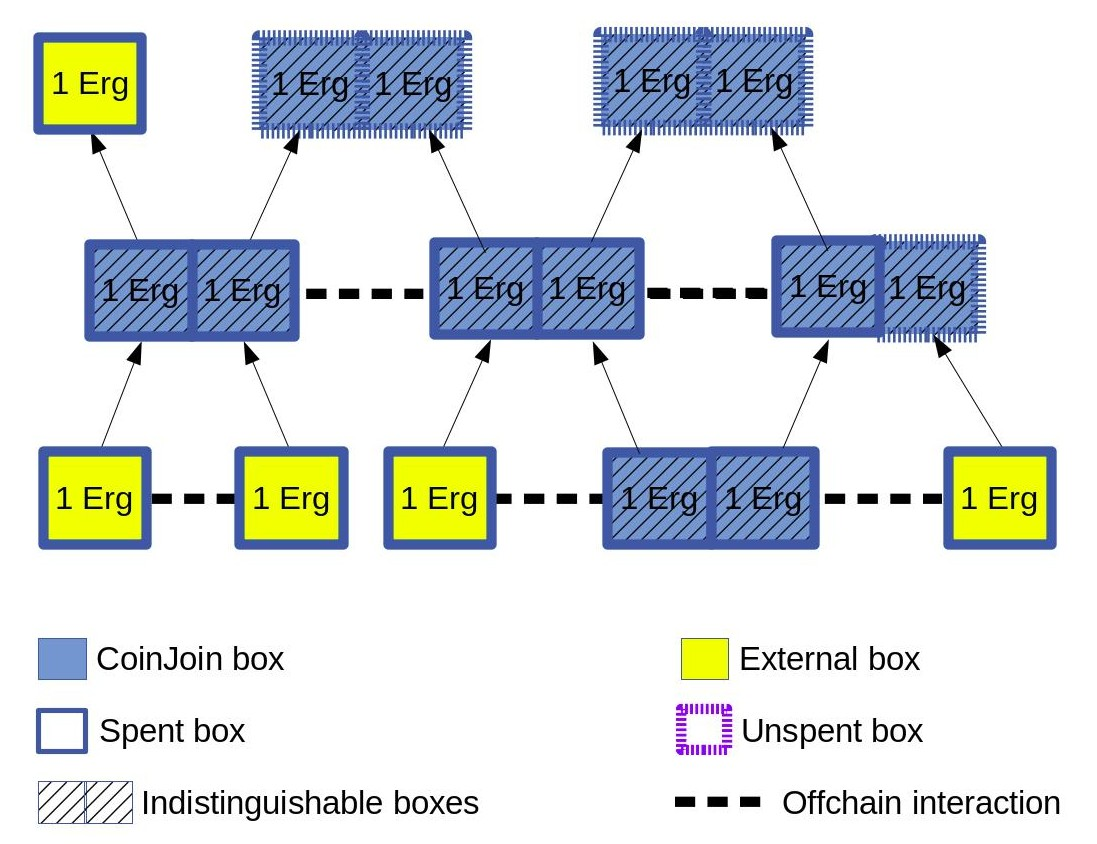
\includegraphics[width=\linewidth]{CoinJoin.jpg}
	\end{subfigure}%
	\caption{Canonical Multi-stage CoinJoin}
	\label{fig:coinjoin}
\end{figure}

In this model, each CoinJoin transaction has exactly two inputs (the boxes at the tail of the arrows) and two outputs (the boxes at the head of the arrows). Creating such a transaction requires a private off-chain interaction between the two parties supplying the inputs, which is denoted by the dashed line. We will ignore fee for now and revisit this issue in Section~\ref{fee}.
The key idea of CoinJoin is that the two output boxes are {\em indistinguishable} in the following sense. 
\begin{enumerate}
    \item The owner of each input box controls exactly one output box.
    \item An outsider has no idea which output corresponds to which input.
\end{enumerate}

Thus, each CoinJoin transaction provides 50\% unlinkability. The output box can be used as input to further CoinJoin transactions and the process repeated to increase the unlinkability to any desired level. We will use the same concept in \algname. 
CoinJoin requires off-chain interaction and this interactive nature is the primary drawback of CoinJoin, which \algname aims to overcome. 

\subsection{\zerocoin}
\label{zerocoin} 

\zerocoin is a privacy enhancing protocol depicted in Figure~\ref{fig:zerocoin}. The protocol uses a pool of coins called the {\em unspent-box pool} (U-pool), to which an ordinary coin is added as a commitment $c$ to secret $s$ using randomness $r$. The coin is later spent from this pool such that the link to $c$ is not publicly visible. The value $c$ must be permanently stored in the U-pool, since the spending transaction cannot reveal it. Instead, it reveals the secret $s$ (also called the {\em serial number}) along with a zero-knowledge proof that $s$ was used in a some commitment in the U-pool. The commitment scheme is such that revealing $s$ does not leak any information about $r$. Thus, the randomness $r$ remains secret. To prevent double spending, the serial number is also stored in another data structure called the {\em spent-box pool} (S-pool). A coin can be spent from the U-pool only if the corresponding serial number does not exist in the S-pool. 

\begin{figure}[h]
	\centering
	\begin{subfigure}{.7\textwidth}
		\centering
		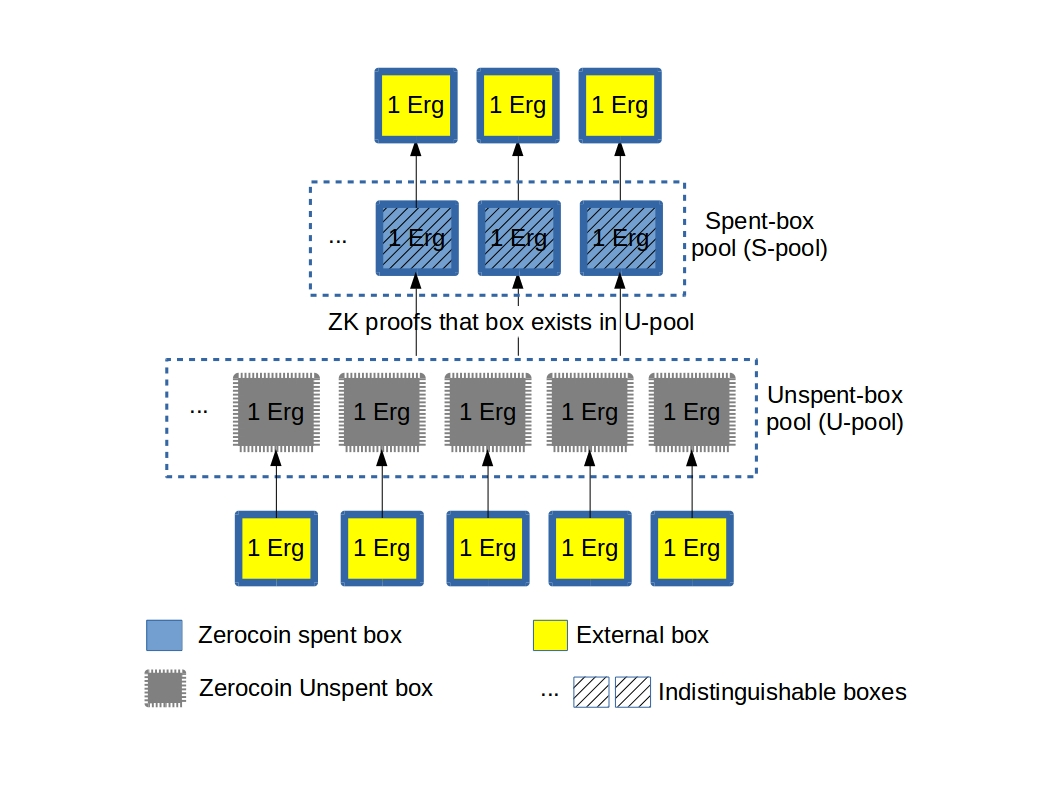
\includegraphics[width=\linewidth]{Zerocoin.jpg}
	\end{subfigure}
	\caption{\zerocoin protocol}
	\label{fig:zerocoin}
\end{figure}

One consequence of this is that both the U-pool (the set of commitments) and the S-pool (the set of spent serial numbers) must be maintained in memory for verifying every transaction. 
Another consequence is that the sizes of the these two sets increase monotonically. 
This is the main drawback of \zerocoin (also Zcash~\cite{zcash}), which \algname tries to address. 
In \algname, once a box is spent, no information about it is kept in memory, and in particular no data sets of monotonically increasing sizes are maintained. 

Considering the addition of a coin to the mix as a deposit and removal as a withdraw, the in-memory storage in \algname is proportional to the number of deposits minus the number of withdraws, while that in ZeroCash is proportional to the number of deposits plus the number of withdraws.  

\subsection{Sigma Protocols} 

Let $G$ be a cyclic multiplicative group where decision Diffie-Hellman (DDH) problem is hard. 
\algname uses two interactive proofs in this setting. 

The first, a variation of Schnorr signatures~\cite{Sch91}, is a {\em proof of knowledge of Discrete Logarithm} of some $u$ to base $g$, where the prover proves knowledge of $x$ such that $u = g^x$. This is called \texttt{proveDlog($g, u$)} and implemented as follows:
\begin{enumerate}
	\item The prover, $\mathcal{P}$, picks $r \stackrel{R}{\leftarrow} \mathbb{Z}_q$ and sends $t = g^r$ to the verifier, $\mathcal{V}$.
	\item $\mathcal{V}$ picks $c \stackrel{R}{\leftarrow} \mathbb{Z}_q$ and sends $c$ to $\mathcal{P}$.
	\item $\mathcal{P}$ sends $z = r + cx$ to $\mathcal{V}$, who accepts iff ${g}^z = t\cdot {u}^c$. 
	
\end{enumerate}

A protocol with this structure $(\mathcal{P} \stackrel{t}{\rightarrow}\mathcal{V}, \mathcal{P} \stackrel{c}{\leftarrow}\mathcal{V}, \mathcal{P} \stackrel{z}{\rightarrow}\mathcal{V})$ is called a sigma protocol if it satisfies {\em special soundness} and {\em honest-verifier zero-knowledge}~\cite{Dam10}. 

The statement to be proved (example ``I know the discrete logarithm of $u$ to base $g$'') is denoted by $\tau$.
Any sigma protocol can be made non-interactive via the Fiat-Shamir transform~\cite{fiatshamir} by setting $c= H(t)$ where $H$ is a hash function. 

As shown in \cite{CDS94}, any two sigma protocols for arbitrary statements $\tau_0, \tau_1$ can be efficiently composed to a single sigma protocol that proves knowledge of one of the witnesses without revealing which. Let $b \in \{0, 1\}$ be such that $\mathcal{P}$ knows the witness of $\tau_{b}$ but not $\tau_{1-b}$. 
$\mathcal{P}$ simulates the proof of $\tau_{1-b}$ to get an accepting transcript $(t_{1-b}, c_{1-b}, z_{1-b})$ and generates $t_b$ properly. $\mathcal{P}$ sends $(t_0, t_1)$ to $\mathcal{V}$. On receiving $c$, $\mathcal{P}$ computes $c_b = c \oplus c_{1-b}$ and then uses $t_b, c_b$ to compute the response $z_b$ properly. Finally $\mathcal{P}$ sends $(z_0, z_1, c_0, c_1)$ to $\mathcal{V}$, who accepts iff both $(t_0, c_0, z_0)$ and $(t_1, c_1, z_1)$ are accepting transcripts and $c = c_0 \oplus c_1$.
We call such a construction the $\ornode$ operator. 

The second primitive we need is a {\em proof of knowledge of Diffie-Hellman Tuple}, where the prover proves knowledge of $x$ such that $u = g^x$ {\em and} $v = h^x$ for generators $g, h$.
This is called \texttt{proveDHTuple}($g, h, u, v$) and implemented using two parallel runs of the first protocol:

\begin{enumerate}
	\item $\mathcal{P}$ picks $r \stackrel{R}{\leftarrow} \mathbb{Z}_q$ and sends $t = ({g}^r, {h}^r)$ to $\mathcal{V}$.
	\item $\mathcal{V}$ picks $c \stackrel{R}{\leftarrow} \mathbb{Z}_q$ and sends $c$ to $\mathcal{P}$.
	\item $\mathcal{P}$ sends $z = r + cx$ to $\mathcal{V}$ who accepts iff ${g}^z = {t_0}\cdot {u}^c$ and $h^z=t_1\cdot v^c$.
\end{enumerate}

We can also define \texttt{proveDHTuple}($g, u, h, v$), the {\em dual} of the above, as a sigma protocol where $\mathcal{P}$ proves knowledge of $y$ such that $h = g^y$ and $v = u^y$.


\section{\algname Protocol}

\algname uses a pool of {\em Half-Mix} boxes. The set of all unspent Half-Mix boxes is called the {\em H-pool}. To mix an arbitrary box $B$, one of the following is done:
\begin{enumerate}
	\item \textbf{Pool:} Add $B$ to the H-pool and wait for someone to mix it.
	\item \textbf{Mix:} Pick any box $A$ from the H-pool and a secret bit $b$. Spend $A, B$ to 
	output two boxes $O_b$ and $O_{1-b}$ spendable by $A$'s and $B$'s owners respectively.
\end{enumerate}

Privacy comes from the fact that boxes $O_b$ and $O_{1-b}$ are indistinguishable so any outsider can only guess $b$ with probability $\frac{1}{2}$. Thus, the probability of guessing the original box after $n$ mixes is $\frac{1}{2^n}$. The protocol is depicted in Figure~\ref{fig:mixname}. 

\begin{figure}[h]
	\centering
	\begin{subfigure}{.7\textwidth}
		\centering
		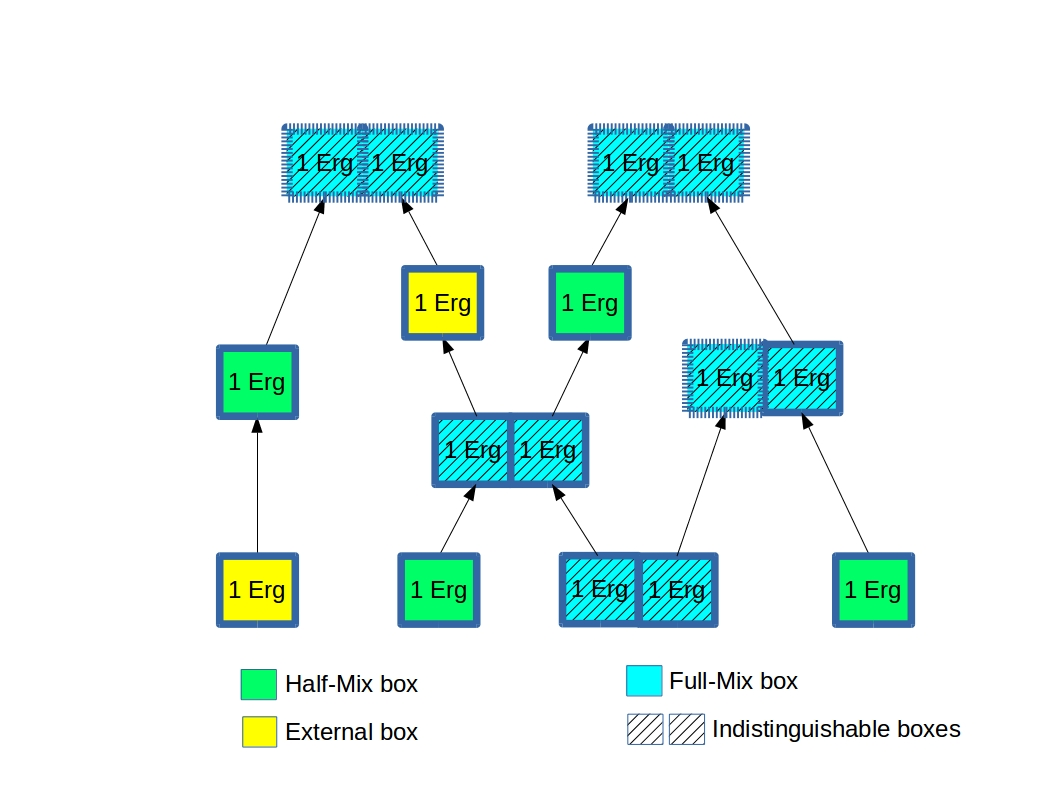
\includegraphics[width=\linewidth]{ZeroJoin}
	\end{subfigure}
	\caption{Multi-round \algname}
\label{fig:mixname}
\end{figure}

\subsection{One \algname Round}
Each individual \algname round consists of two stages, the {\em pool} followed by the {\em mix} stage. 
Let $g$ be some generator of $G$ that is fixed beforehand. Each box has optional registers ${\alpha}, {\beta}$ that can store elements of $G$.

We will encode the protocol at the the smart contract layer using a sufficiently advanced language that allows us to specify predicates on the entire transaction. 
In other words, we require a language that supports context level C2 or higher as defined in~\cite{bypassing}. The smart contract (or the guard script) of a box specifies the conditions under which it can be spent. 

Without loss of generality, Alice will pool and Bob will mix. 

\begin{enumerate}
	\item \textbf{Pool:} To add a coin to the H-pool, Alice picks a secret $x\in \mathbb{Z}_q$ and creates a box $A$ containing $u = g^x$ and a certain guard script (described below). The box is now considered added to the pool. 
	\item \textbf{Mix:} Bob picks a box, say $A$, uniformly from the pool. He also picks secrets $(b, y) \in \mathbb{Z}_2\times \mathbb{Z}_q$. He spends $A$ with some of his own boxes to create two output boxes $O_0, O_1$ of equal value such that:
	\begin{enumerate}
		\item Registers $({\alpha}, {\beta})$ of $O_b$ and $O_{1-b}$ store $(g^y, u^y)$ and $(u^y, g^y)$ respectively. 
		\item $O_b, O_{1-b}$ are protected by the sigma statement given below:
    		\begin{equation}\label{fullScriptEqn}
    		    \texttt{proveDHTuple}(g, {\alpha}, u, {\beta})~\ornode~\texttt{proveDlog}(g, {\beta})
    		\end{equation}
	\end{enumerate}
\end{enumerate}

$O_b$ and $O_{b-1}$ can be spent by Alice and Bob respectively using their secrets. Alice can identify her box as the one with ${\beta} = {\alpha}^x$. 
Assuming that the DDH problem is hard, no outsider can guess $b$ with probability better than $\frac{1}{2}$. 

%\textbf{Enforcing Bob's correct behavior:} 
The above protocol works assuming Bob behaves correctly. 
We can encode other rules in the protocol or the smart contract of $A$ that enforce Bob to behave correctly most of the time.
For instance, we can enforce Bob to create two outputs with registers $\alpha, \beta$ swapped and that both outputs have the same value as $A$. However,
since the DDH problem is hard, we cannot test whether the values in the registers are of the correct form (i.e., one is $g^y$ and other is $u^y$).
This is where the dual of \texttt{proveDHTuple} for secret $y$ will come to our rescue. 
Concretely, the script of $A$ must enforce the following rules for Bob:

	\begin{enumerate}
		\item Bob must create two outputs $O_0, O_1$ with the same value as $A$. 
		\item Both $O_0, O_1$ must be protected by the script of Eq.~\ref{fullScriptEqn}
        \item Let $i_j$ be register $i$ of $O_j$. Then the following must hold: 
            \begin{equation}\label{outputRegs}
    		({\alpha}_0, {\beta}_0) = ( {\beta}_1, {\alpha}_1)
            \end{equation}
		\item Bob must prove (via the dual) that either $(g, u, {\alpha}_0, {\beta}_0)$ or $(g, u, {\beta}_0, {\alpha}_0)$ is of the form $(g, g^x, g^y, g^{xy})$. In other words, Bob must prove the sigma statement: 
    		\begin{equation}\label{bobCondition}
    		\texttt{proveDHTuple}(g, u, {\alpha}_0, {\beta}_0)~\ornode~\texttt{proveDHTuple}(g, u, {\beta}_0, {\alpha}_0)
    		\end{equation}
		
	\end{enumerate}
	
\subsection{Analysis}

For correctness, Alice requires that no one should be able to spend $A$ in a manner that makes the resulting output(s) unspendable by her.

First note that due to Eqs.~\ref{outputRegs} and~\ref{bobCondition}, Bob has no choice but to create two outputs $O_0, O_1$ such that the registers $({\alpha}, {\beta})$ of $O_b$ and $O_{1-b}$ contain $(g^y, g^{xy})$ and $(g^{xy}, g^y)$ respectively for some integer $y$ and bit $b$. Then the spending condition of Alice's Full-Mix box, $O_b$, reduces via Eq.~\ref{fullScriptEqn} to:
$$\texttt{proveDHTuple}(g, g^{y}, g^x, g^{xy}) ~\ornode~ \texttt{proveDlog}(g, g^{xy}).$$ 

The above statement can be proven by anyone who knows at least one of $x$ or $xy$. 
Thus, Alice can spend this because she knows $x$. 

For Alice's soundness, no one else apart from her should have the ability to spend $O_b$. Assume that there exists such a spender. Since only Alice knows $x$ and the only other way to spend the box is via $\texttt{proveDlog}(g, g^{xy})$, that other spender must know $xy$. Such a spender cannot know $y$ and so cannot spend $O_{1-b}$. We can model this spender as a black-box taking as input $(g, g^x)$ and outputting $(g^y, xy)$ for some $y\neq 0$. Since such a black-box can be used to solve the Computational Diffie-Hellman (CDH) problem in $G$, we can rule out this possibility.

From Bob's point of view, the spending condition of $O_{1-b}$ reduces to 
$$\texttt{proveDHTuple}(g, g^{xy}, g^x, g^{y}) ~\ornode~ \texttt{proveDlog}(g, g^{y}).$$
Since Bob knows $y$, he can spend the box using the right part of the statement. Finally, if someone apart from Bob spends $O_{1-b}$ then they must have used the left part of the statement because using the right part would require knowledge of $y$. However, using the left part is not possible because $(g, g^{xy}, g^x, g^{y})$ is not a valid Diffie-Hellman tuple. Hence, no one else apart from Bob can spend $O_{1-b}$. Note that despite the left being an invalid tuple, the simulator must generate a valid proof for it, otherwise we could use the simulator to solve DDH.

For privacy, the only difference between $O_b$ and $O_{1-b}$ is that registers $({\alpha},{\beta})$ are of the form $(g^y, g^{xy})$ and $(g^{xy}, g^y)$ respectively. Assuming that the Decision Diffie-Hellman (DDH) problem in $G$ is hard, no outsider has the ability to distinguish the boxes before they are spent. Since each box is spent using a sigma $\ornode$ proof that is zero-knowledge~\cite{Dam10}, this applies even after they are spent. 

\paragraph{Comparing with CoinJoin and \zerocoin:} Both CoinJoin and \algname use two indistinguishable outputs that provide the privacy (see Section~\ref{coinjoin}). However, each CoinJoin transaction requires an off-chain interaction over a private channel. In \algname, this interaction is replaced by a public transaction on the blockchain. 

%Note that CoinJoin supports {\em covert} mode, where the use is concealed.

Both \zerocoin and \algname add boxes to a pool and later spend them via zero-knowledge proofs (see Section~\ref{zerocoin}). 
The difference is that the privacy in \zerocoin depends on the size of the pool, while that in \algname depends on the number of rounds. Thirdly, \zerocoin's pool increases monotonically in size, while that of \algname does not. Finally, the NIZK proofs in \zerocoin are much larger compared to the non-interactive sigma proofs of \algname. 

\subsection{Implementing \algname In \langname}
\label{impl}
Each round of \algname is a two-stage protocol (pool followed by mix). One way to implement \algname would be to create a specialized blockchain just for this purpose that has the protocol hardwired (as was done, for example, in Zcash~\cite{zcash}). However, this limits the use of the blockchain. 

A more pragmatic way is to encode \algname as a smart contract on top of a general-purpose UTXO blockchain such as Ergo~\cite{ergo} using the concepts from \cite{multistage}, that is, by encoding \algname as a two-stage protocol with the `fingerprint' of the second stage embedded within a smart contract of the first stage.
In the approach of~\cite{multistage}, Alice's box $A$ encodes the protocol by enforcing the structure of Bob's spending transaction. 
This is done as follows. 

For brevity, assume that \texttt{alpha}, \texttt{beta}, \texttt{gamma} are aliases for the registers $\alpha, \beta, \gamma$ of a box that contain elements of $G$. We already saw the first two used earlier. The third is to store $u$. We give some more notation below. 
\begin{enumerate}
    \item \texttt{script} refers to the guard script (in binary format) of the box.
    \item \texttt{value} refers to the quantity of Ergo's primary token stored in the box. 
    \item \texttt{id} refers to the globally unique identifier of the box. 
    \item \texttt{SELF} is omitted, so \texttt{id} on its own, for example, must be read as \texttt{SELF.id}. 
\end{enumerate}

Let $x$ be Alice's secret and let $u = g^x$. To create the Half-Mix box with $u$, first compile the following script of the second stage to get \texttt{fullMixScript}:
{\small
\begin{Verbatim}[frame=single]
// Contract #1: contract for Full-Mix box (fullMixScript)
proveDHTuple(g, alpha, gamma, beta) || proveDlog(g, beta)
\end{Verbatim}
}
Next create a script, \texttt{halfMixScript}, with the following code:
{\small
\begin{Verbatim}[frame=single]
// Contract #2: contract for Half-Mix box (halfMixScript)
INPUTS(0).id == id &&
OUTPUTS(0).alpha == OUTPUTS(1).beta && 
OUTPUTS(0).beta == OUTPUTS(0).alpha && 
OUTPUTS(0).gamma == gamma && OUTPUTS(1).gamma == gamma &&
OUTPUTS(0).value == value && OUTPUTS(1).value == value &&
OUTPUTS(0).script == fullMixScript &&  
OUTPUTS(1).script == fullMixScript &&
OUTPUTS(0).alpha != OUTPUTS(0).beta &&      // prevent y = 0
(proveDHTuple(g, gamma, OUTPUTS(0).alpha, OUTPUTS(0).beta) || 
 proveDHTuple(g, gamma, OUTPUTS(0).beta, OUTPUTS(0).alpha))
\end{Verbatim}
}

Note that \texttt{OUTPUTS(0)} is the first output of the transaction, \texttt{OUTPUTS(1)} is the second output, and so on. Alice's box $A$ is protected by \texttt{halfMixScript}. Alice must store $u$ in register \texttt{gamma} of that box.


\section{\mixname: \algname with Fee}
\label{fee}

Similar to \zerocoin and CoinJoin (Figure~\ref{fig:coinjoin}), each Half-Mix and Full-Mix box in \algname must hold the same fixed value, which is carried over to the next stage. This implies zero-fee transactions because any fee must either be paid from the Full/Half-mix boxes (which breaks the fixed value requirement) or from a non-\algname box (which breaks privacy). Zero-fee transactions are not practical. 

Here we describe how to handle fee on the Ergo blockchain. To differentiate the generic protocol (\algname) from the underlying implementation using Ergo, we give the name {\em \mixname} to any of the various extensions in this section that are largely specific to Ergo. 
We classify \algname transactions into the following:

\begin{enumerate}
    \item \textbf{Alice entry:} When someone plays the role of Alice to create a Half-Mix box and add to the H-pool. The inputs to the transaction are one or more non-\mixname boxes ({\em external} boxes) and the output is one Half-Mix box. 
    \item \textbf{Bob entry:} When someone plays the role of Bob to spend a Half-Mix box and remove from the H-pool. The other inputs of the transaction are one or more non-\mixname boxes and the outputs are two Full-Mix boxes. 
    \item \textbf{Alice or Bob exit:} When someone plays the role of Alice or Bob to spend a Full-Mix box and send the funds to a non-\mixname box. 
    \item \textbf{Alice or Bob reentry as Alice:} When someone plays the role of Alice or Bob to spend a Full-Mix box and create a Half-Mix box (i.e., send the coin back to the H-pool). The input is a Full-Mix box and the output is a Half-Mix box of the same amount.
    \item \textbf{Alice or Bob reentry as Bob:} When someone plays the role of Alice or Bob to spend a Full-Mix box along with another Half-Mix box and create two new Full-Mix boxes. The input is a Half-Mix box and a Full-Mix box and the outputs are two new Full-Mix boxes.
\end{enumerate}

Clearly, for both Alice and Bob entries, fee is not an issue because both parties can fund the fee component of the transaction from a known source. Similarly for case 3, when exiting the system, part of the amount in the Full-Mix box can be used to pay fee. The only time we need to hide the source of fee is when we spend a Full-Mix box and want to reenter as either Alice or Bob. 

\subsection{An Altruistic Approach}
\label{donation}

In this approach, fee is paid by a {\em sponsor} when spending a Full-Mix box for reentry. 
We use a variation of {\em Fee-Emission boxes} presented in~\cite{Fee-Emission}. 

\paragraph{Fee-Emission Box:} A sponsor creates several Fee-Emission boxes to pay reentry fee. Such a box can be spent under the following conditions:

\begin{enumerate}
    \item There is exactly one Fee-Emission box as input.
    \item There is exactly one Full-Mix box as input.
    \item Either exactly one input or exactly one output is a Half-Mix box.
    \item The updated balance is stored in a new Fee-Emission box.
\end{enumerate}

This is encoded in \langname as follows:

{\small
\begin{Verbatim}[frame=single]
// Contract #3: contract for Fee-Emission box
def isFull(b:Box) = hash(b.script) == fullMixScriptHash 
def isHalf(b:Box) = hash(b.script) == halfMixScriptHash
def isFee(b:Box) = hash(b.script) == feeScriptHash
def isCopy(b:Box) = b.script == script && 
                    b.value == value - fee
val asAlice = INPUTS.size == 2 && OUTPUTS.size == 3 &&
              isFull(INPUTS(0)) && isHalf(OUTPUTS(0)) &&
              isCopy(OUTPUTS(1)) && isFee(OUTPUTS(2)
val asBob = INPUTS.size == 3 && OUTPUTS.size == 4 &&
            isHalf(INPUTS(0)) && isFull(INPUTS(1)) &&
            isCopy(OUTPUTS(2)) && isFee(OUTPUTS(3))
asAlice || asBob 
\end{Verbatim}
}

The condition \texttt{asAlice} encodes the rules of spending a Full-Mix box to emulate Alice for the next mix and create a Half-Mix box. Similarly, the condition \texttt{asBob} has the rules for spending a Full-Mix box as Bob's contribution in a mix. 

The sponsor pays the fee whenever a Full-Mix box is remixed. However, there is no guarantee that some given Full-Mix box was actually created in a mix transaction. The only way to determine this is to examine the transaction that created the box. However, this is not yet possible in \langname. Thus, the above approach is susceptible to freeloaders who store their funds in a Full-Mix box. However, such freeloaders must either create a Half-Mix box or spend another Half-Mix box, thereby forcing them participate in the protocol. This gives no advantage to freeloaders who still need to pay fee to create a fake full-mix box. 

\subsection{Mixing Tokens}

Ergo's primary token is known as {\em Erg}, which is necessary to pay for transaction fees and storage rent~\cite{chepurnoy2018systematic}. An Ergo transaction conserves primary tokens (they can neither be created nor destroyed) and any box must have a positive quantity of primary tokens.
Each box can optionally have {\em secondary tokens} which are uniquely identified by an id. Unlike primary tokens, an Ergo transaction can destroy secondary tokens. Additionally, each transaction can also create (i.e., {\em issue}) at most one new token in arbitrary quantity, whose id is the globally unique id of the first input box box of that transaction. 

In this approach, we will still use a Fee-Emission box (as in Section~\ref{donation}) to pay the fee in Ergs. However, we will also use secondary tokens issued by the creator of the Fee-Emission box, which we call {\em mixing tokens} (identified by \texttt{tokenId}). The Fee-Emission box can only be used by destroying a mixing token.

\paragraph{Approximate Fairness:} We use the approximate fairness strategy described in~\cite{advtutorial}. At a high level the idea is as follows.
Each mix transaction consumes one mixing token, which must be supplied by the inputs. Thus, there must be at least one mixing token among the inputs. Additionally, to keep the outputs indistinguishable, each must have the same number of tokens. 

The approximate fairness strategy says that Bob must supply half the token, and is allowed to supply less tokens than Alice as long as both started with the same amount and Bob lost them in sequential mixes.
The approximate-fairness strategy works only if two conditions are satisfied. The first is that mixing tokens are confined within the system by restricting their transfer to only those boxes that participate in a remix. 
The second is to ensure that tokens always enter the system in a fixed quantity, and that too in one of the two \mixname boxes. 

\subsection{Token Confinement}

In this section we enforce the first requirement of approximate fairness, that of confining the tokens within the system. 
Recall that the Half-Mix box's script refers to the Full-Mix box's script via the constant \texttt{fullMixScriptHash}. Our approach additionally requires the Full-Mix box's script to refer back to the Half-Mix box's script. We do this by storing the hash of the Half-Mix script in one of the registers of the Full-Mix box. Let \texttt{delta} be an alias for this register that stores an array of bytes. The scripts are also modified.

\paragraph{Fee-Emission Box:}
We modify \texttt{isFull} method of the Fee-Emission box contract:

{\small
\begin{Verbatim}[frame=single]
// Contract #4: contract for Fee-Emission box
def isFull(b:Box) = hash(b.script) == fullMixScriptHash && 
                    b.delta == halfMixScriptHash
(... remaining code same as Contract #3)                    
\end{Verbatim}
}

Recall that the rule for spending the Fee-Emission box is to destroy one mixing token. While the above contract does not directly enforce this requirement, it does so indirectly via the Full-Mix and Half-Mix scripts discussed below.

\paragraph{Full-Mix Box:}

Modify \texttt{fullMixScript}, the contract of a Full-Mix box as well:

{\small
\begin{Verbatim}[frame=single]
// Contract #5: contract for Full-Mix box
def isHalf(b:Box) = hash(b.script) == delta && 
                    b.value == value
def isFull(b:Box) = b.script == script &&
                    b.delta == delta && b.value == value
def noToken(b:Box) = b.tokens(tokenId) == 0
val nextAlice = isHalf(OUTPUTS(0)) && INPUTS(0).id == id
val nextBob = isHalf(INPUTS(0)) && INPUTS(1).id == id
val destroyToken = OUTPUTS.forall(noToken)
val nextAliceLogic = OUTPUTS(0).tokens(tokenId) == 
                     INPUTS(0).tokens(tokenId) - 1 && 
                     OUTPUTS(0).tokens(tokenId) > 0

((nextAlice && nextAliceLogic) || nextBob || destroyToken) 
&& (... earlier condition from Contract #1)
\end{Verbatim}
}

The script enforces the transfer of mixing tokens when spending the Full-Mix box to create a Half-Mix box. In particular, the tokens can only be transferred if the transaction either outputs a Half-Mix box (i.e., the spender takes the role of Alice in the next mix step, in which case one mixing token is destroyed) or participates in a mix transaction as Bob and spends a Half-Mix box along with this Full-Mix box (in which case, the transfer of mixing tokens is governed by the contract in the Half-Mix box).
% The usage of mixing tokens when spending the Full-Mix box in a mix transaction is enforced in the Half-Mix box. In the remaining cases the mixing tokens must be destroyed.  

\paragraph{Half-Mix Box:}
Next, the Half-Mix contract (\texttt{halfMixScript}) is also modified:
{\small
\begin{Verbatim}[frame=single]
// Contract #6: contract for Half-Mix box
val alice = INPUTS(0).tokens(tokenId)
val bob = INPUTS(1).tokens(tokenId)
val out0 = OUTPUTS(0).tokens(tokenId)
val out1 = OUTPUTS(1).tokens(tokenId)
val tLogic = alice + bob == out0 + out1 + 1 && bob > 0 && alice > 0 
  
OUTPUTS(0).delta == hash(script) && 
OUTPUTS(1).delta == hash(script) && out0 == out1 && tLogic &&
&& (... earlier condition from Contract #2)
\end{Verbatim}
}

The above contract assumes that the boxes already have some quantity of mixing tokens and enforces how these must be used. Each mix transaction is assumed to consume one such token, and to maintain privacy, the token balance must be equally distributed between the two outputs. The contract follows the {\em approximate-fairness} strategy where Alice requires Bob to contribute at least one mixing token~\cite{advtutorial}. For {\em perfect fairness} add the condition \texttt{alice == bob}. 

\subsection{Token Entry}

\paragraph{Token-Emission Box:} A Token-Emission box is used to get mixing tokens for entry into the system as either Alice or Bob. It contains the following contract. 

{\small
\begin{Verbatim}[frame=single]
// Contract #7: contract for Token-Emission box
def isCopy(b:Box) = b.script == script && b.value == value &&
                    b.tokens(tokenId) == tokens(tokenId) - amt
def isFull(b:Box) = hash(b.script) == fullMixScriptHash && 
                    b.delta == halfMixScriptHash
def isHalf(b:Box) = hash(b.script) == halfMixScriptHash
def isFee(b:Box) = hash(b.script) == feeScriptHash &&
                   b.value == fee
def isEntry(b:Box) = (isFull(b) || isHalf(b)) && 
                     b.tokens(tokenId) == amt
def isZero(b:Box) = b.tokens(tokenId) == 0

INPUTS(0).id == id && isZero(INPUTS(1)) && INPUTS.size == 2 &&
isEntry(OUTPUTS(0)) && isCopy(OUTPUTS(1)) && isFee(OUTPUTS(2))
\end{Verbatim}
}

% The Token-Emission box 
% is the final piece of the puzzle and 
% encodes the following logic. 
Anyone can spend the Token-Emission box to send a fixed amount \texttt{amt} of mixing tokens to either a Half-Mix box or a (fake) Full-Mix box, which should be the first output of the transaction. The other outputs are a copy of the token-emission box with the balance tokens and the fee paying output. The transaction must have exactly two inputs, with the token-emission box being the first and the second containing zero mixing tokens. 

We can use mixing tokens to verify that a given Full-Mix box was indeed created in a mix transaction, and a given Half-Mix box was indeed created by spending a Full-Mix box. In particular, this is true if and only if the box contains less than \texttt{amt} and more than 0 mixing tokens.  

While the above Token-Emission box gives the mixing tokens for free, it is trivial to modify the contract to sell the tokens at some given rate. The only change required is in the \texttt{isCopy} method:

{\small
\begin{Verbatim}[frame=single]
// Contract #8: contract for Token-Emission box
def isCopy(b:Box) = b.script == script && 
                    b.value == value + amt * rate &&
                    b.tokens(tokenId) == tokens(tokenId) - amt
(... remaining code same as Contract #7)
\end{Verbatim}
}

We also want the token issuer to be able to withdraw any Ergs deposited by token buyers. To achieve this, the token-emission box is again modified:

{\small
\begin{Verbatim}[frame=single]
// Contract #9: contract for Token-Emission box
(... earlier condition from Contract #8) || 
(issuerPubKey && INPUTS.size == 1 && 
 OUTPUTS(0).script == script && OUTPUTS(0).value > minErgs &&
 OUTPUTS(0).tokens(tokenId) == tokens(tokenId))
\end{Verbatim}
}
It is necessary to keep a certain amount of Ergs, \texttt{minErgs} inside each Token-Emission box, otherwise the box may be destroyed when miners collect storage rent. This value should be large enough to ensure sustenance for several years. 
In order to allow several people to buy tokens in the same block and to avoid collisions when multiple people try to spend the same token-emission box, there must be several token-emission boxes. 

\paragraph{Analysis:} 
Because of the condition \texttt{bob > 0} in \texttt{tLogic} of the Half-Mix box, a mix transaction requires Bob to supply at least one token, and since these tokens can only be stored in either Full or Half-Mix boxes, the second input of a mix transaction must be a Full-Mix box (as opposed to any box).
That Full-Mix box can either be the output of a mix transaction (a real Full-Mix box) or the output of a token purchase transaction (a fake Full-Mix box).

Another consequence of \texttt{bob > 0} is that at least one token must exist in order to spend Alice's box. In the case that mixing tokens become unavailable, Alice's box is rendered unspendable. In order to handle this, we need to ensure that mixing tokens are always available. One way would be to have each token-emission box store a large number of tokens, much more than what can be purchased with all the available Ergs. Before storing any funds in a Half-Mix box, it must be ascertained that there are a large number of mixing tokens stored in at least one token-emission box. 

An alternate way to ensure that Alice's Half-Mix box does not get stuck due to non-availability of tokens would be to allow Alice to spend the box using her secret. This requires modifying the Half-Mix box as follows:

{\small
\begin{Verbatim}[frame=single]
// Contract #10: contract for Half-Mix box
def noToken(b:Box) = b.tokens(tokenId) == 0

(proveDlog(g, alpha) && INPUTS.size == 1 && OUTPUTS.forall(noToken)) || 
(... earlier condition from Contract #6)
\end{Verbatim}
}

The above modification allows Alice to spend the Half-Mix box using her secret but she must destroy all mixing tokens in doing so. 

Figure~\ref{fig:mixingtokens} gives an example flow with the above contracts in place. To avoid clutter, we skipped the fee output in the above flow. However, each transaction is implicitly assumed to have an additional box for paying fee.

\begin{figure}[h]
	\centering
	\begin{subfigure}{0.9\textwidth}
		\centering
		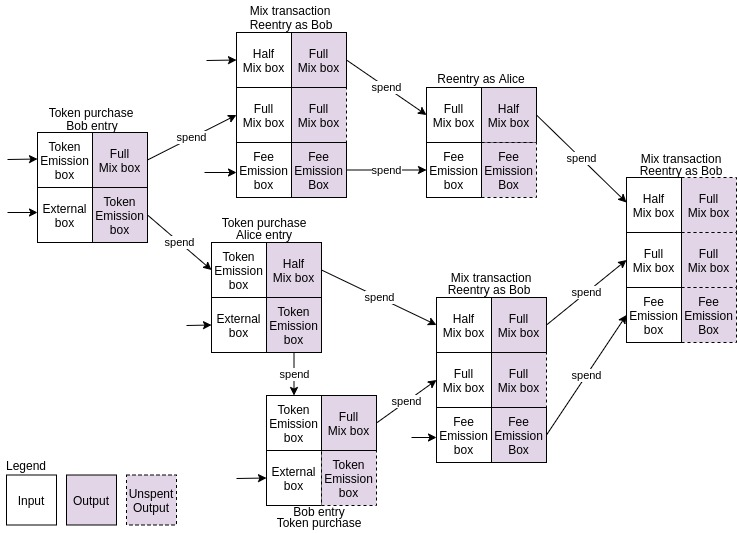
\includegraphics[width=\linewidth]{MixingTokens.jpg}
	\end{subfigure}
	\caption{Multi-round \mixname with Mixing Tokens to handle fee}
\label{fig:mixingtokens}
\end{figure}

A mix transaction is always a reentry as Bob and both Alice and Bob's entry is through a token purchase transaction. 

The predicate \texttt{alice > 0} also requires that the Half-Mix box have at least one token, implying that the only way to create the Half-Mix box would be in a token purchase transaction or transaction for reentry as Alice. In particular, it is impossible to create a Half-Mix box in an other manner.

\bibliographystyle{unsrt}
\bibliography{main}
\end{document}
